\chapter{Simulation} % (fold)
\label{prt:simulation}
\section{Introduction} % (fold)
\label{cha:sim_introduction}
To help design and analysis experiments MuSIC was simulated, this was used both to design the detectors and understand the data that they have produced. Two core simulations were created, one using G4Beamline (G4BL) and the other using Geant4. 

The G4BL simulation was mainly used to simulate the bulk of MuSIC and the hadron interactions. A more detailed and configurable Geant4 simulation was used to simulate the detectors. This section will discuss the general features of Geant4 and G4BL before a more detailed discussion of the actual implementation. The discussion will focus on the work done on the Geant4 simulation for the fifth MuSIC beam time as this was the most complete simulation performed. Simulations were used in earlier beam but not to the same extent, most notably the G4BL simulation was used to interpret the total charged particle flux measurements. Less simulation work was done for the muon lifetime measurement as it was often simpler to compare the measured lifetimes with those made by others.

\section{Geant4} % (fold)
\label{sec:geant4}
Geant4 is described as `a toolkit for the simulation of the passage of particles through matter'~\cite{Geant4 REF}. Rather than a complete program it is a collection of pre-compiled libraries that comprise the basics required to simulate various interactions. It has additional libraries that provide further functionality such as visualisation. 

Geant4 is written in C++ using an object orientated approach that allows the user to either use Geant4's implementation of a class or write their own. This flexibility also means that all the functionality of Geant4 is explicitly opt-in making the resultant programs much faster than they would otherwise be (as only the components that are selected are used). Geant4's speed does come at a cost which is that a larger amount of configuration is required than would be needed for less flexible solutions (c.f.\ G4BL).

Even with it's increased flexibility Geant4 has certain requirements that must be met in order to work. These requirements embody the minimum information to create a simulation they define what to simulate, where to simulate it and which processes to simulate. Geant4's base requirement is that there is an instance of one of each of three classes\footnote{Whilst there is a technical distinction between an instance of a class (an object) and the class itself for the sake of clarity the word `class' is used throughout.}:
\begin{description}
  \item[The detector constructor] A description of the detector.
  \item[The physics list] The physics processes to use.
  \item[The primary action generator] Information describing the initial particle to simulate.
\end{description}
With these three classes defined a simple program can be linked against the Geant4 libraries and will run. The libraries will use the primary action generator to create the initial particle; simulate its movement and interactions as described by the physics list in the world specified by the detector constructor. In addition to these required components a simulation can be further refined with custom classes that replace or expand those supplied by Geant4.

The rest of this section will consider the roles of the detector constructor, physics list and primary action generator. The detector constructor will be treated separately to the other two classes as it is a primarily static description. Discussion of the physics list and primary action generator will be rolled together with several other key concepts under the execution model which covers the dynamic aspects of the simulation.

% subsection material_simulation (end)
\subsection{Detector Constructor} % (fold)
\label{sub:detector_constructor}
The detector constructor has several two key jobs: defining the materials and defining the volumes of the detector. The materials describe the physical properties of various elements, compounds and mixtures. The volumes describe the position, rotation, material and logical attributes of the detector. 

\subsubsection{Material Properties} % (fold)
\label{ssub:material_properties}

The material properties in Geant4 can be thought of as members of one of two sets: referred to here as `core' and `extended'. The core properties cover those values that are required for reasonable calculations of energy loss in the material, the extended properties cover more detailed calculations and properties that are more specialised.

The core properties for an element are the atomic number, the mass number and the molar density. Compounds and mixtures are described as ratios of their component elements at a specific density. Extended properties can be any property of the material that the user is interested in, for our purposes these were the optical properties of the materials and are discussed below.

Due to the computationally complex nature of interactions between light and material Geant4 doesn't implement them by default. When enabled Geant4 uses single values or tables of values to describe the various optical processes that it can simulate. The tables it uses are defined in terms of photon energy and missing values are generated via interpolation. 
% subsubsection material_properties (end)

\subsubsection{Detector Volumes} % (fold)
\label{ssub:detector_volumes}

The detector volumes describe the physical pieces of the detector. Each volume is split between three classes: the shape, the logical volume and the physical volume. The shape describes the geometrical volume. The logical volume describes how the piece works within the larger simulation. Finally the physical volume places and orientates the volume. 

The volume's shape is normally described by either basic polyhedra (cubes, tubes, trapezoids etc.) Geant4 also provides basic tools for creating compound shapes made of the intersection, difference and addition of basic shapes. Using these tools it's possible to create suitably complex constructions in code. Geant4 does offer more powerful tools (e.g.\ geometry importing) but these were not used for this simulation.

The logical volume stores the specific attributes of the component. The main information that the logical volume maintains is what material a component is (this can be changed using messengers) and what shape it is. A single logical volume can be associated with many physical volumes to make repetitive constructs easy to define.

As has been noted the physical volume positions the component. Additionally it stores which logical volume this component is in (as well as which logical volume describes it). Storing the parent volume means that a single logical volume can contain many sub-components to make bulk manipulation easier, as all placements are done with respect to the parent volume's origin.

% subsubsection detector_volumes (end)
\subsection{Execution model} % (fold)
\label{sub:execution_model}

Geant4 manages simulation by splitting it into several layers. At the top-most level is the run, this represents a collection of events and all the associated information (e.g.\ the detector configuration). Each event within a run starts with an initial particle (as defined by the primary action generator) and tracks it through the detector, if another particle is produced (e.g.\ if the initial particle decays or scatters) then a new track is added to the simulation to represent the new particle(s). A track is made up of steps, each step represents a period of time in which nothing `significant' occurs.

A `significant' occurrence is one which will make further calculations of properties of the particle difficult and therefore limit the length of the particle's step. Determination of this step length is split between multiple classes within Geant4 but they can be broadly separated into four categories: detector considerations, user imposed limits, continuous physical processes and discrete physical processes. In each category the method is broadly the same, any class that can have an affect on the particle proposes a distance from the current position at which the affect will occur, e.g.\ a detector may report that the particle will leave the current volume in 10~mm whilst a decay process may report that the particle will likely decay in 5~mm. Once all the proposed step lengths have been determined the shortest is found and the particle is transported that distance and properties (position, time, energy, particle type(s)\footnote{Should the particle decay it is replaced at the end of the step with the appropriate daughter particles.} etc.) are updated. 

As has been stated the main consideration for the step length with respect to the detector are the volume boundaries which generally delimitate a change in material that will obviously determine which processes occur and how. Other detector considerations include the affect of a fields on the particles transport. Continuous processes generally only limit a particle by reducing its energy to zero (obviously some processes can increase it but these rarely limit a step length). Discrete processes obviously limit a particle by changing it in some way, for example by having a particle decay. Once a step length has been determined any continuous affects are applied to the particle, if it's at a volume boundary it moves into the next volume, any limiting discrete processes are applied and the next step length is calculated. 

The processes (discrete or continuous) are supplied by the physics list. The physics list registers which processes can occur to which particles and then assigns a class to handle that eventuality. In this way physical processes can be enabled or disabled at will. It is also possible to register several classes to a single particle-process pair in order to describe different situations the most common use of this is to apply different models depending on particle energy. Obviously the full range of physical processes that need to be described to accurately simulate the standard model is quiet large, luckily Geant4 has extensive pre-compiled lists that cover the major types of particle interaction as well as several specialised lists that cover specific situations e.g.\ low energy regimes which are often ignored in high energy simulations as they can be computationally expensive. 

% subsection execution_model (end)
% section geant4 (end)
%%%%%%%%%%%%%%%%%%%%%%%%%%%%%%%%%%%%%%%%%%%%%%%%%%%
\section{G4beamline} % (fold)
\label{sec:g4beamline}
G4beamline (G4BL) is a program written by Muons, Inc.~\cite{G4BL ref}, it is a particle tracking simulation program that uses Geant4. Unlike Geant4, G4BL is a pre-compiled program that the user writes simple scripts that define the parameters of the simulation. In general creating simulations in G4BL is much quicker than Geant4 as a significant amount of `boilerplate' code is removed at the cost of flexibility. The use of Geant4, rather than G4BL, for the detector simulation was mainly driven by the finer control Geant4 offered.

% section g4beamline (end)
%%%%%%%%%%%%%%%%%%%%%%%%%%%%%%%%%%%%%%%%%%%%%%%%%%%
% chapter sim_introduction (end)
\section{Implementation} % (fold)
\label{cha:implementation}
As has been discussed the simulation was split between G4BL and Geant4. This section will focus on the implementation of the Geant4 detector simulation as this constituted the bulk of the work carried out.

\subsection{G4Beamline} % (fold)
\label{sec:g4beamline_impl}
G4BL was used to describe the bulk of MuSIC: the pion capture solenoid: target, capture solenoid, the shielding and return yoke; and the transport solenoids: bending magnets and pipe sections. A virtual detector, with radius 50~cm, was placed at the end of the beam pipe and recorded the particles that pass through it. A wireframe rendering of the set up can be seen in figure~\ref{fig:images_Geometry_g4bl_wireframe}. 

\begin{figure}[hptb]
  \centering
    \includegraphics[width=.9\textwidth]{images/Geometry/g4bl_wireframe.png}
  \caption{Wireframe of the G4BL simulation of MuSIC. The dark red is the iron yoke, the bright red are the solenoids, the light blue is the pion capture solenoid shielding and the yellow line is a simulated proton.}
  \label{fig:images_Geometry_g4bl_wireframe}
\end{figure}

Using this script G4BL simulated the computationally expensive hadronic interactions at the production target. The output of the G4LB simulation could then be reused for multiple detector set ups by importing the particle distribution into Geant4.

G4BL was used to simulate 900~million initial protons the beam from which was used as input for the Geant4 simulation. At the end of the beam-pipe this gave the total charged particle distribution as seen in figure~\ref{fig:images_sim_2d_charged_particle_flux}, figure~\ref{fig:images_sim_2d_per_pid_flux} shows the break down of the flux based by particle type. Table~\ref{tab:g4bl_particle_counts} shows the number of each particle type and the rate of production per proton. 

The evolution of the final distribution is shown in figure~\ref{fig:images_pid_counts_in_beamline} with the position of the monitors used shown in figure~\ref{fig:images_g4bl_monitor_locations_bigger_edit}. 

\begin{figure}[hptb]
  \centering
    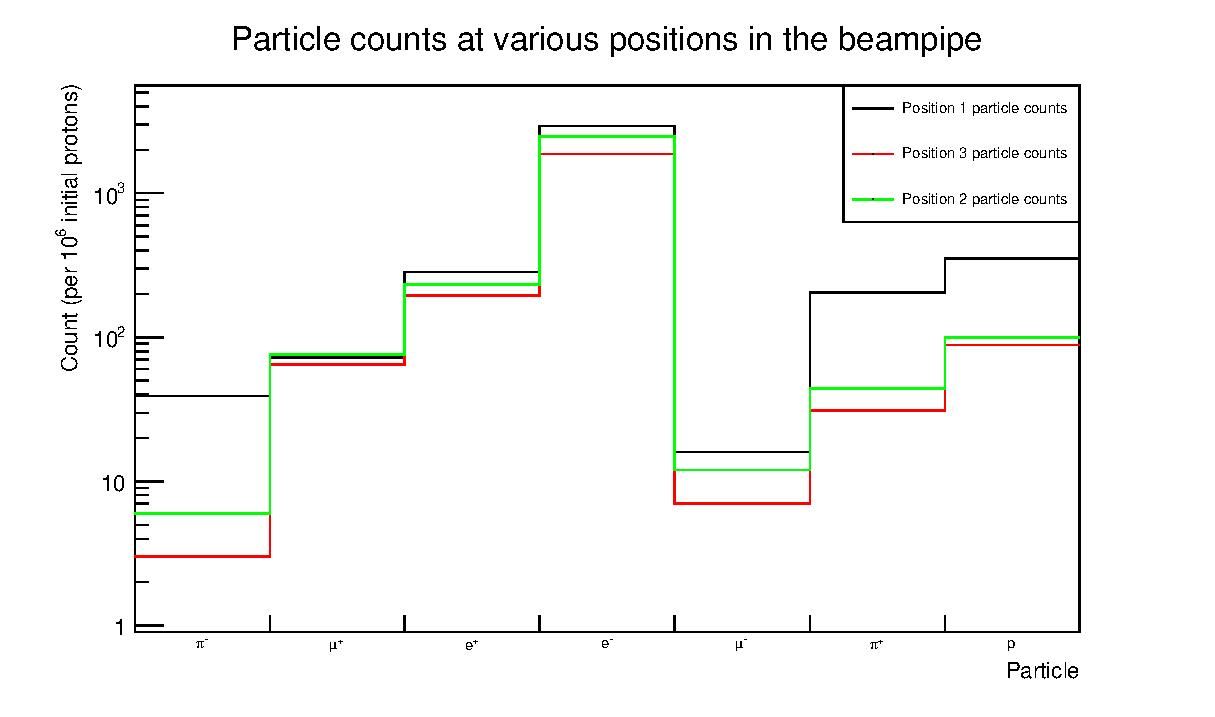
\includegraphics[width=.9\textwidth]{images/pid_counts_in_beamline.eps}
  \caption{Evolution of the particle distribution in the G4BL simulation of MuSIC. Position 1 is 1~cm after the pion capture solenoid and positions 2 and 3 are after the first dipole and at the end of the beam pipe respectively.}
  \label{fig:images_pid_counts_in_beamline}
\end{figure}

\begin{figure}[hptb]
  \centering
    \includegraphics[width=.9\textwidth]{images/g4bl_monitor_locations_bigger_edit.png}
  \caption{Position of the beam monitors used to track the particle distribution through the G4BL simulation. Note: the monitors used to create the distribution used in the final Geant4 simulation have a much smaller, 50~cm, radius compared to 2~m used in this image (as the smaller radius monitors would not be visible).}
  \label{fig:images_g4bl_monitor_locations_bigger_edit}
\end{figure}

\begin{figure}[hptb]
  \centering
  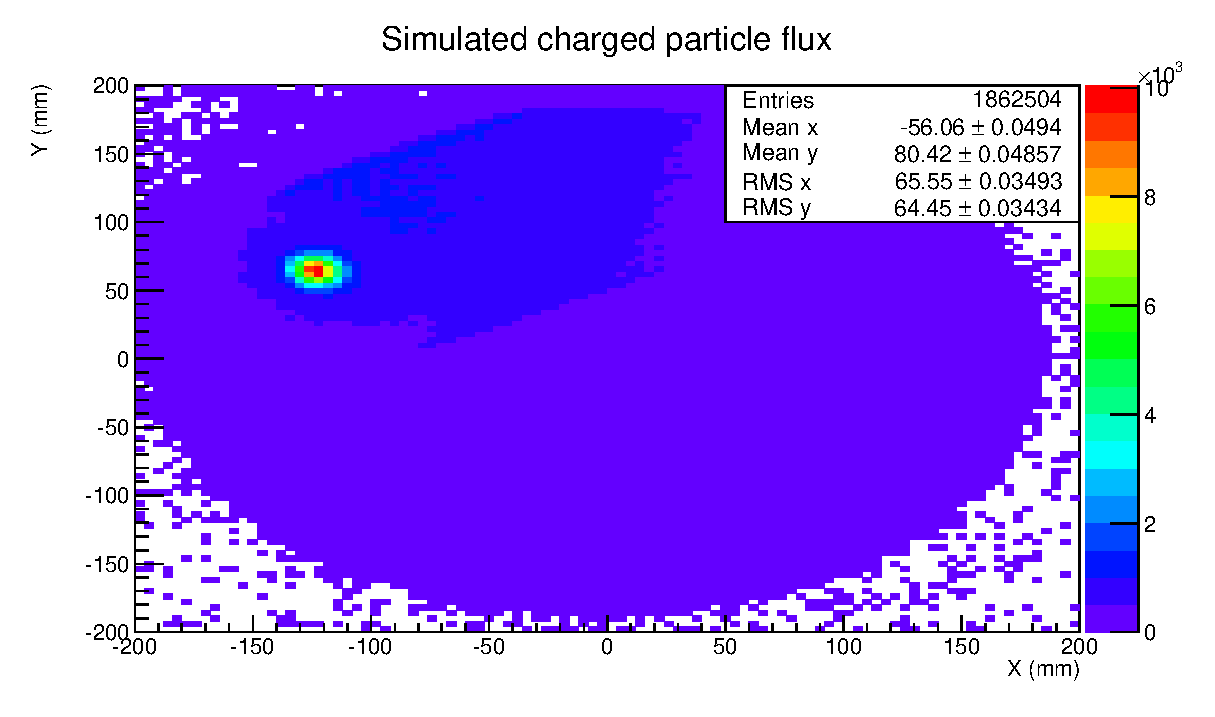
\includegraphics[width=.9\textwidth]{images/sim_2d_charged_particle_flux.eps}
  \caption{Total charged particle flux at the end of the MuSIC beam-pipe.}
  \label{fig:images_sim_2d_charged_particle_flux}
\end{figure}

\begin{sidewaysfigure}
  \centering
    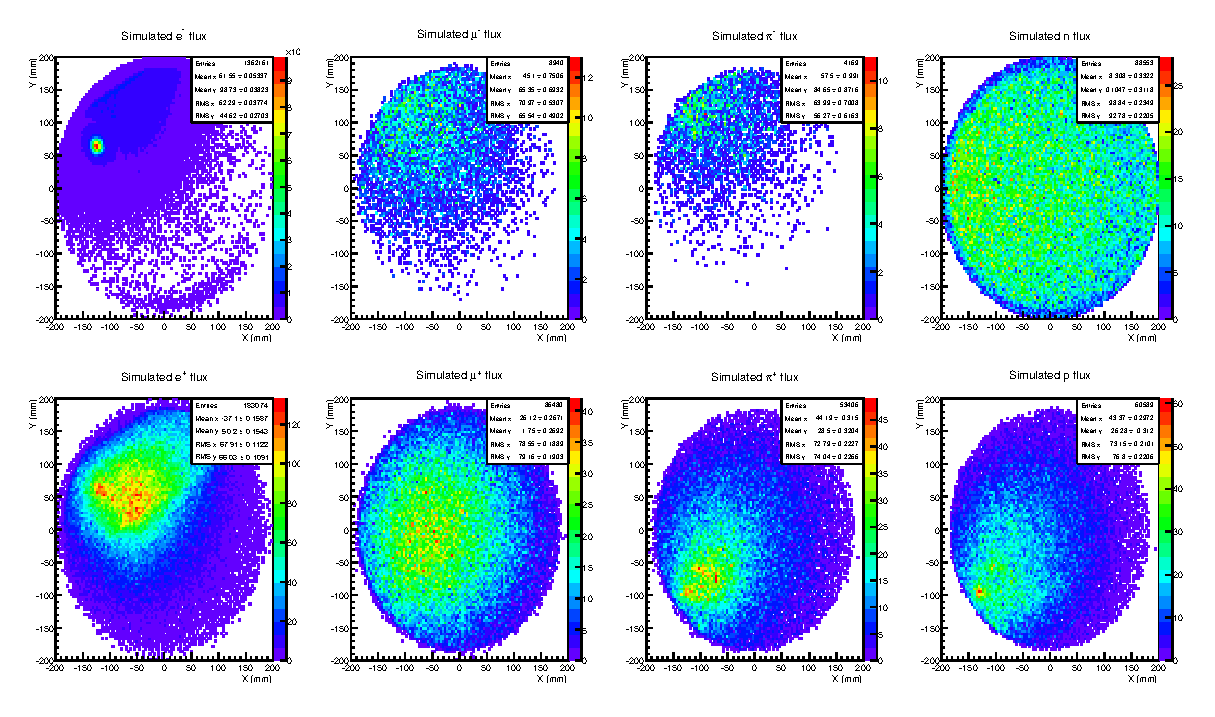
\includegraphics[width=.9\textwidth]{images/sim_2d_per_pid_flux.eps}
  \caption{Distributions of the different charged particles across the beam-pipe.}
  \label{fig:images_sim_2d_per_pid_flux}
\end{sidewaysfigure}

\begin{table}
  \begin{center}
  \begin{tabular}{c | r | c | c}
    \multicolumn{1}{c|}{\multirow{2}{*}{Particle}} 
               &  \multicolumn{1}{c|}{\multirow{2}{*}{Count}} 
                             &  \multicolumn{2}{c}{Mean position (mm)}    \\
               &             &  Horizontal  &  Vertical \\
    \hline
      e\(^-\)  &  1,438,537  &    \(-\)62   &       99  \\
      e\(^+\)  &    209,069  &    \(-\)37   &       50  \\
    \(\mu^-\)  &      9,009  &    \(-\)45   &       65  \\
    \(\mu^+\)  &     86,710  &    \(-\)26   &   \(-\)2  \\
    \(\pi^-\)  &      4,206  &    \(-\)58   &       85  \\
    \(\pi^+\)  &     53,528  &    \(-\)44   &  \(-\)29  \\
       p       &     61,445  &    \(-\)43   &  \(-\)26  \\
  \end{tabular}
  \end{center}
  \caption{General information of the charged particle distributions at the end of the MuSIC beam-pipe.}
  \label{tab:g4bl_particle_counts}
\end{table}

% section g4beamline (end)
\subsection{Geant4} % (fold)
\label{sub:geant4}
The Geant4 simulation was split into several key classes in addition to the detector constructor, primary action generator and physics list previously discussed. These classes were:
\begin{description}
  \item[The magnetic field] which gave the field strength within the detector.
  \item[The stepping action] which analysed every step of a particle's track and if it passed certain criteria, passed the track to ROOT for recording.
  \item[ROOT] which read and wrote ROOT files that were used to import the G4BL distribution and record events from the stepping action.
  \item[The messengers] a set of classes for configuring the simulation without re-compiling the program.
\end{description}
The implementation of each of these classes will now be discussed with the exception of the ROOT and messenger classes which primarily implemented utilities and had no impact upon the simulation or the data it produced.

The messengers were used to specify parameters to be used in the following run. These parameters are supplied via configuration files called macros. Four aspects of the simulation were controlled via macros: the primary action generator, the physics list, the magnetic field and the detector constructor. It was then possible to write further scripts that generated macros to test a range of configurations, e.g.\ a script was used to generate several macros that ran the simulation with a range of different degrader thicknesses.

% subsection geant4 (end)
\subsection{Detector Constructor} % (fold)
\label{sec:detector_constructor}
The detector constructor is by far the most complex of the classes used in the simulation. The implementation of the detector construction was split over several functions, this discussion will follow similar lines. The materials will be discussed, then the optical properties and finally the geometry of the detector.

\subsubsection{Materials} % (fold)
\label{ssub:implementation_materials}

To simulate the detectors at MuSIC a fairly simple selection of materials were required, the elemental metals used for the stopping target and degrader; and several plastics that made up the scintillators. Geant4 treats materials as either pure elements or as mixtures (even if they're a compound). For the materials used at MuSIC only six elements were needed (H, C, N, O, Al and Cu), these had their standard values~\cite{Some reference for elements} for mass number, atomic number and, where needed, density. The majority of these were used as components of plastics and for approximating the composition of air but copper and aluminium were used in their pure form (hence the inclusion of their density). 

The compounds and mixtures (table~\ref{tab:sim_compounds_and_mixtures}) were, with the exception of air, components of the scintillators. Mylar was used to wrap the scintillators; EJ-212 (a trade name for NE-102A) is the core scintillating material; and BCF-91A is the Wave-Length Shifting (WLS) fibre, which has a polystyrene core with a PMMA cladding. The optical properties that were included in the simulation were:
\begin{enumerate}
  \item The refractive index, n.
  \item The emission spectrum that described the scintillation light produced by ionising particles.
  \item Absorption spectrum, used in concert with an additional emission spectrum this described the WLS fibres.
  \item Scintillation yield, for EJ-212 this was 10,000~MeV\(^{-1}\) as stated by the manufacturer and assumes a linear response.
\end{enumerate}
These properties were only implemented for the materials involved in the optical system. The emission and absorption spectra for the scintillator and WLS fibres were approximated to the curves given in the material data sheets (\cite{EJ_212} and \cite{BCF_91A}), the values used are plotted in  figures~\ref{fig:images_ej-212-g4}~and~\ref{fig:images_bcf-91a-g4} respectively.

\begin{table}
  \begin{center}
  \begin{tabular}{c | c | c | d{4} | c | c}
    Compound/  &  \multirow{2}{*}{Components}  
                               &  \multirow{2}{*}{Ratio}
                                           &  \multicolumn{1}{c|}{Density}
                                                   & Refractive
                                                        &  \multirow{2}{*}{Ref}  \\
    Element    &               &           &  \multicolumn{1}{c|}{(g/cm\(^3\))}
                                                   &  Index 
                                                           &        \\
    \hline
    Air        &     N, O      &    7:3    &  1.290  &  1.00  & \cite{Air}        \\
    Mylar      &   H, C, O     &  8:10:4   &  1.397  &   --   & \cite{Mylar Data} \\
    EJ-212     &     H, C      &  1:1.103  &  1.023  &  1.58  & \cite{EJ212}      \\
    BCF-91A (core)  &  H, C    &  1:1.006  &  1.05   &  1.60  & \cite{BCF_91A}    \\
    BCF-91A (clad)  & H, C, O  &   8:5:2   &  1.05   &  1.49  & \cite{BCF_91A}    \\
    
  \end{tabular}
  \end{center}
  \caption{Compounds and mixtures used for the simulation. No refractive index is given for mylar as it's opaque. An additional property of EJ-212 was the light yield which was 10,000~MeV\(^{-1}\).}
  \label{tab:sim_compounds_and_mixtures}
\end{table}

\begin{figure}[hptb]
  \centering
    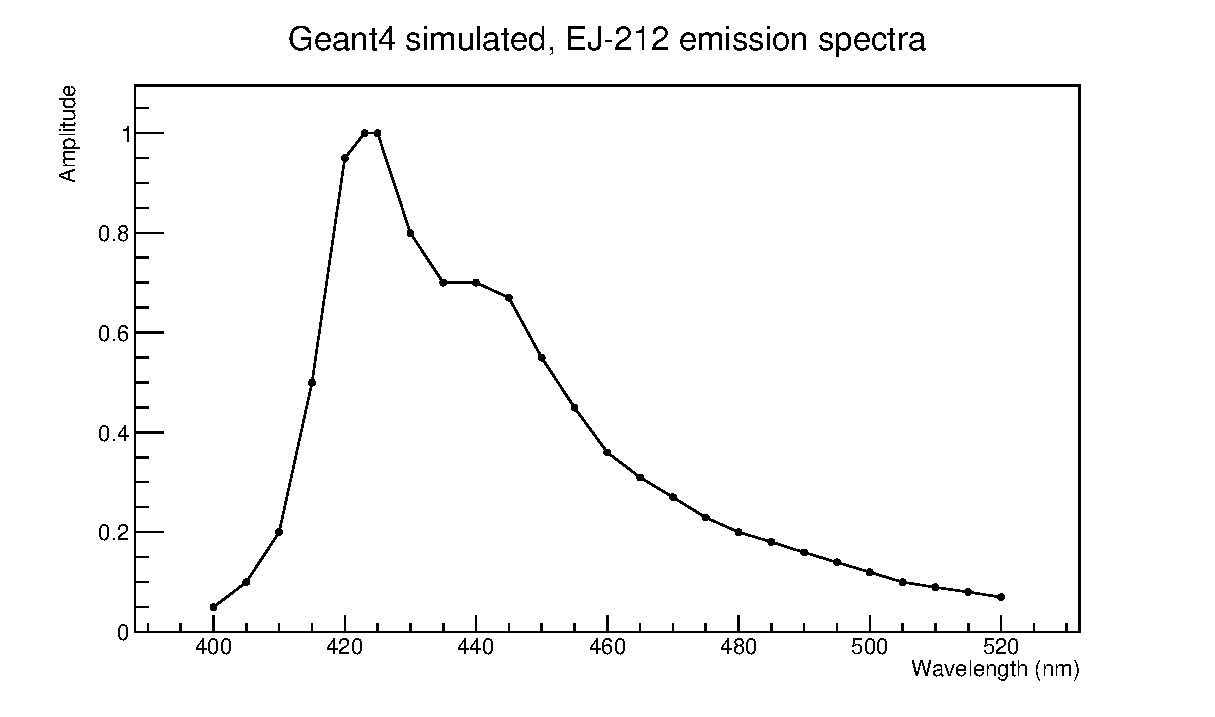
\includegraphics[width=.9\textwidth]{images/ej-212-g4.eps}
  \caption{Scintillation spectra for EJ-212. The points represent the values passed to Geant4 and are based on those read from the manufacture's data-sheet~\cite{EJ_212}}
  \label{fig:images_ej-212-g4}
\end{figure}


\begin{figure}[hptb]
  \centering
    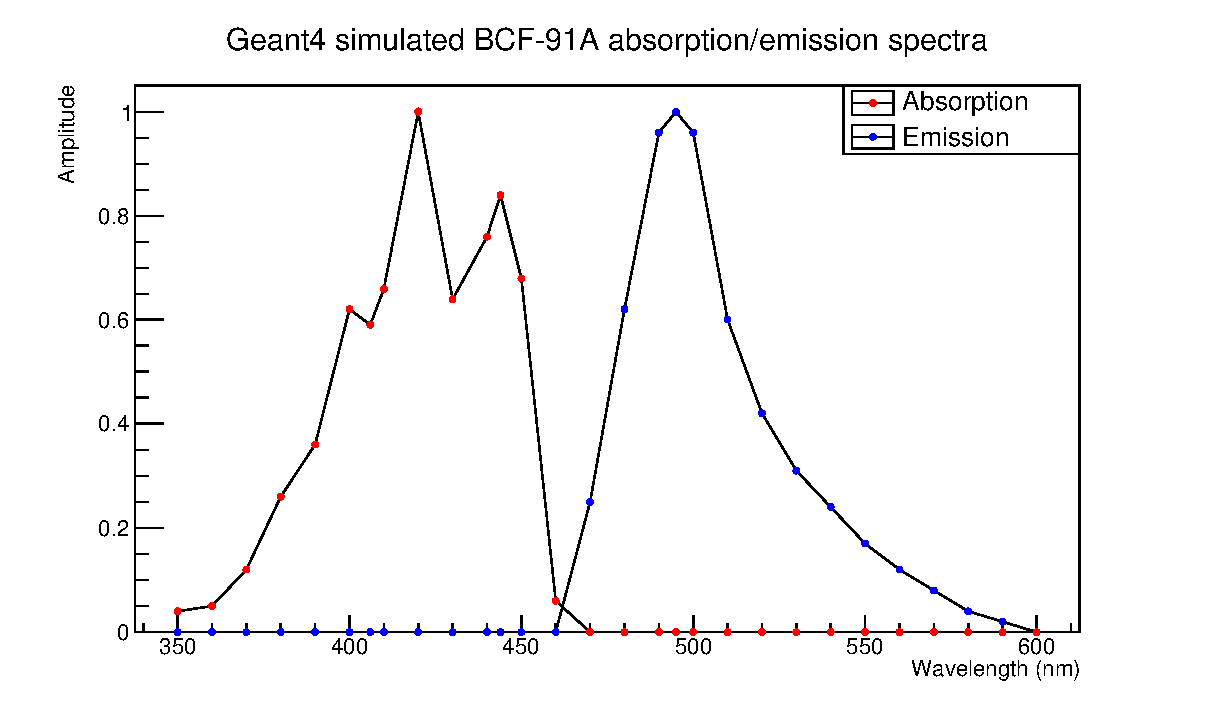
\includegraphics[width=.9\textwidth]{images/bcf-91a-g4.eps}
  \caption{Absorption and re-emission spectra for BCF-91A wavelength shifting fibre. The points represent the values used in Geant4 to approximate the manufacture's curve as given in the data-sheet~\cite{BCF-91A}.}
  \label{fig:images_bcf-91a-g4}
\end{figure}

% subsubsection implementation_materials (end)
\subsubsection{Detector geometry} % (fold)
\label{ssub:implementation_detector_geometry}

MuSIC was simulated as an \(8\times8\times8\)~m\(^3\) volume of air containing the detector. The size of the volume was chosen to simplify transformations of the detector with respect to the magnetic field. The detector was implemented as four placed volumes inside a single logical volume that allowed all of them to be correctly positioned with respect to the magnetic field. The four sub-volumes were the upstream counter, the downstream counter, the degrader and the stopping target. This was the set-up used for the muon lifetime measurements and the final momentum spectrum measurements made during runs 4 and 5.

The degrader and stopping target were configured so that their material and thickness could be changed using macros. This made testing configurations prior to beam-time much quicker and easier. This also meant that the degrader could be removed by creating a volume of air. The materials used for the degrader and stopping target were simple elemental metals (aluminium and copper respectively). Both components were implemented as simple sheets with the dimensions given in table~\ref{tab:st_and_deg_dimensions}.

\begin{table}
  \begin{center}
  \begin{tabular}{c | c | c | c | c}
    \multirow{2}{*}{Component}
                     &  \multirow{2}{*}{Material} 
                                   &  \multicolumn{3}{c}{Dimension (mm)}  \\
                     &             &   X   &   Y   &       Z       \\
    \hline
    Stopping Target  &  Copper     &  370  &  310  &      0.5      \\
    Degrader         &  Aluminium  &  400  &  400  & 0, 0.5, 1, 5  \\
    
  \end{tabular}
  \end{center}
  \caption{Dimensions of the stopping target and degraders. The degrader width of 0~mm is when the degrader is removed and replaced with air. The Z~axis is the main beam direction with the X and Y axes being in the horizontal and vertical directions respectively.}
  \label{tab:st_and_deg_dimensions}
\end{table}

The counters were more complex. Each counter was split into a number of `paddles' (eight upstream, five downstream). A paddle was composed of a main scintillator, a 45\(^{\circ}\) section of pipe (also made of scintillator material) that mimicked the optical cement and a length of wavelength shifting fibre (made of a core and shell). Mylar was then used to define an optical surface that existed at the boundary between scintillator and air. An optical surface is a special construct in Geant4 that is not a full volume but a set of physical affects that occur when optical photons move from one volume to the next, in this way the reflective affect of mylar wrapping was created. A \(1\times1\times1\)~mm\(^3\) volume of air is placed at the end of each wavelength shifting fibre to act as a Multi-Pixel Photon Counter (MPPC) detector region. A side on view of the layout of a counter can be seen in figure~\ref{fig:images_Geometry_full_strip}, the dimensions used for the paddles are are given in table~\ref{tab:dimensions_of_paddles}. A top down view of the simulation is shown in figure~\ref{fig:images_top_for_combo_with_field}.

\begin{figure}[hptb]
  \centering
    \includegraphics[scale=0.5]{images/Geometry/full_strip.png}
  \caption{Side on view of a counter strip, the square surrounding the wavelength shifting fibre is the MPPC region. }
  \label{fig:images_Geometry_full_strip}
\end{figure}

\begin{figure}[hptb]
  \centering
    \includegraphics[width=.7\textwidth]{images/top_for_combo_with_field.eps}
  \caption{Top-down view of the entire simulation showing the region of interest of the magnetic field overlaying the detector volumes. The interaction is a muon decaying outside of the detector and emitting a positron (the blue line) and two neutrinos (the green lines). Within the region of interest the colour indicates the magnetic field strength (red is high, blue is low).}
  \label{fig:images_top_for_combo_with_field}
\end{figure}

\begin{table}
  \begin{center}
  \begin{tabular}{c | c | c | c}
    Component      & Material         & Number     &  Dimensions (mm\(^3\)) \\
    \hline
    Upstream              &  EJ-212          &  8         &  \(380\times30\times0.5 \) \\
    Downstream            &  EJ-212          &  5         &  \(380\times50\times3.5 \) \\
    WLS fibre (core)      &  BCF-91A (core)  &  1/paddle  &  
                                        \multirow{2}{*}{\(500\times(r=0.5)\)} \\
    WLS fibre (cladding)  &  BCF-91A (clad)  &  1/paddle  &  \\
    MPPC                  &  Air             &  2/paddle  &  \(1\times1\times1 \) \\
  \end{tabular}
  \end{center}
  \caption{Dimensions of the simulated paddle components. The wavelength shifting fibres were the same for both up and down stream counters, as were the `MPPCs'. The WLS fibre's cladding is said to be 3\% of the total diameter so this is what is used.}
  \label{tab:dimensions_of_paddles}
\end{table}

% section detector_constructor (end)
\subsection{Primary Action Generator} % (fold)
\label{sec:primary_action_generator}
The primary action generator is a relatively simple class that specifies the properties of the initial particle to be simulated. This means for all implementations defining the particles type, position within the volume and initial momentum. 

At MuSIC the key task of the primary action generator was to either import the particle distribution from the G4BL simulation or create particles with a distribution similar. The source and type of particle could be configured using messengers.

To import from G4BL the particle type, momentum and position were all read from the root file which G4BL saved them in. Approximations to G4BL were used for basic tests, the approximations were simple gaussian (and double guassian) fits to the G4BL data. It was hoped that the approximations would yield results close enough to the G4BL simulation to be useful but they were not good enough. It was found that the approximated distributions gave significantly different rates for stopping muons in the detector when compared to the G4BL distribution. This difference meant the approximations were only used for general tests of the analysis technique rather than for comparison to measured data. 

% section primary_action_generator (end)
\subsection{Physics List} % (fold)
\label{sec:physics_list}
Geant4 provides the majority of physics processes as precompiled lists that cover the major aspects of a simulation. For MuSIC the key attribute of each list was the accuracy at low energies. In this respect the most important lists were those dealing with electromagnetic processes. To cover this `option3' and the `extra' lists were used which have improved low energy simulations and more detailed processes. Most importantly the `extra' list implements muon capture at rest. The few hadronic processes were simulated with the `HP' QGSP-BERT and the elastic physics models, both of which have better methods for simulating low energy neutrons.

One problem with the default supplied physics lists is that the implementation of mu capture at rest is based mainly on theoretical work that doesn't accurately model the capture rate of muons on copper. This is obviously a problem as copper is the main stopping target used at MuSIC. The lifetime for muonic copper produced using unmodified Geant4 is \(\sim1.2\mu\)s compared to the experimental value of 163.5~ns~\ref{Suzuki et al}. This difference can be seen in figure~\ref{fig:images_mu-_lifetime_in_cu_modded_g4} and figure~\ref{fig:images_mu-_lifetime_in_cu_unmodded_g4} which show the muon decay spectra of negative muons with the modified and un-modified versions of Geant4 respectively. 
\begin{figure}[hptb]
  \centering
    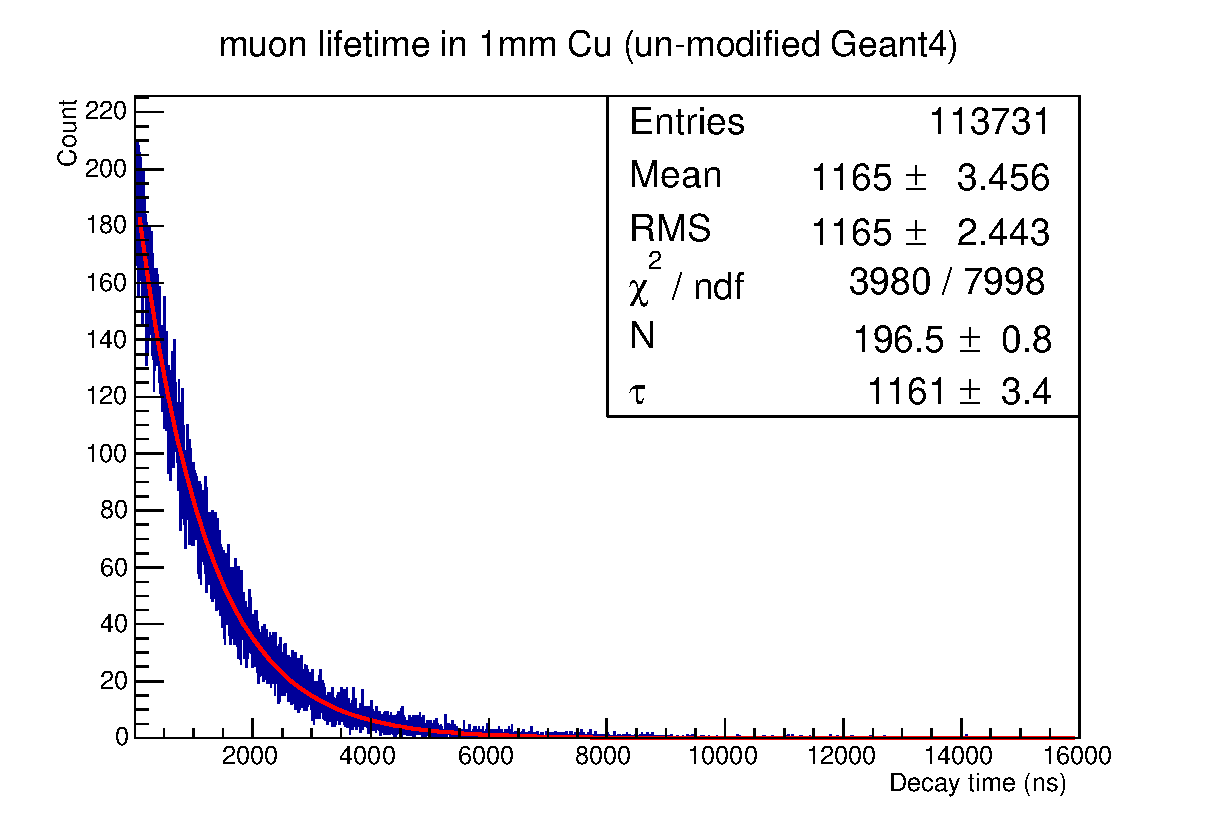
\includegraphics[width=.9\textwidth]{images/mu-_lifetime_in_cu_unmodded_g4.eps}
  \caption{Decay spectrum of \(1\times10^6\) negative muons hitting a 1~mm copper target using an unmodified version of Geant4. The decay times are fitted using \(N_f\exp(-x/\tau_f) +  N_{cu}\exp(-x/\tau_{cu})\). The poor fit for \(\tau_f\) is due to the lack of differentiating power between the free muon lifetime and Geant4's copper lifetime.}
  \label{fig:images_mu-_lifetime_in_cu_unmodded_g4}
\end{figure}

\begin{figure}[hptb]
  \centering
    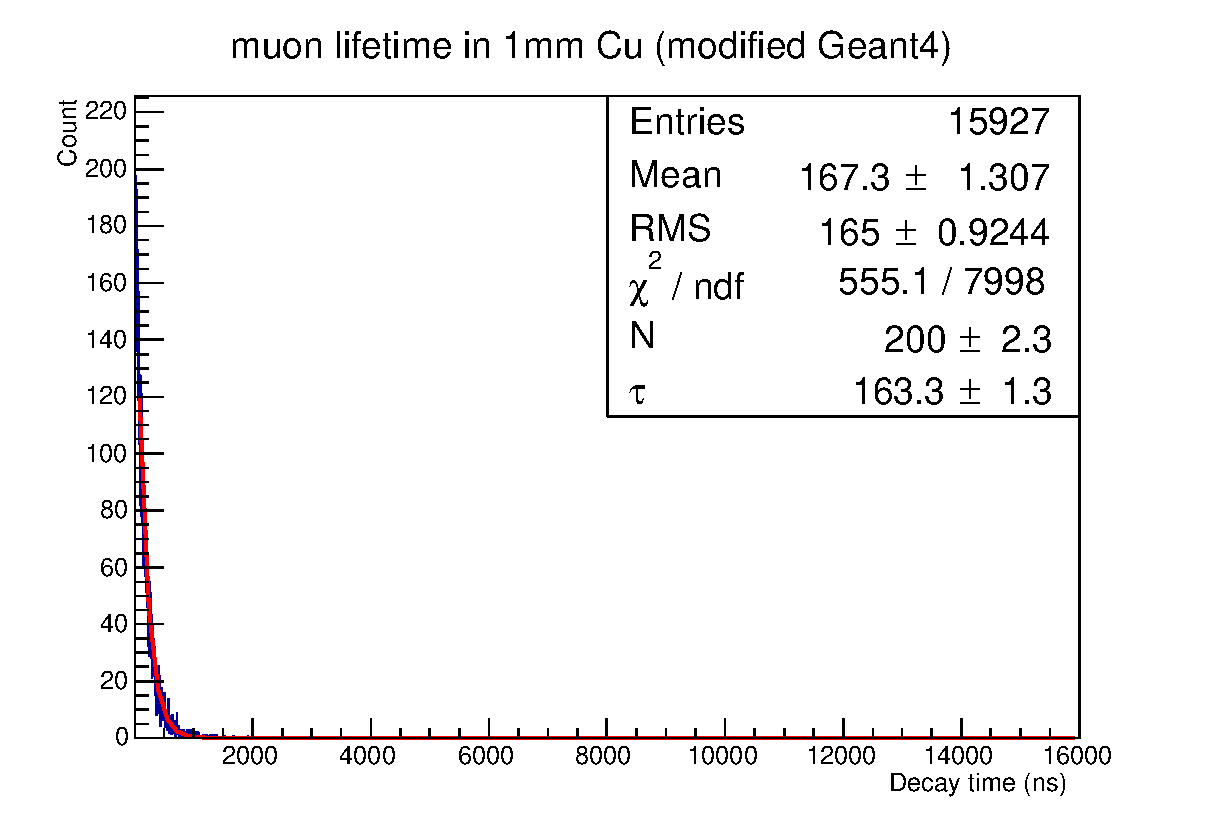
\includegraphics[width=.9\textwidth]{images/mu-_lifetime_in_cu_modded_g4.eps}
  \caption{Decay spectrum of \(1\times10^6\) negative muons hitting a 1~mm copper target using a version of Geant4 modified with the experimental muonic copper lifetime of 163.5~ns. The spectrum is fitted using \(N_f\exp(-x/\tau_f) +  N_{cu}\exp(-x/\tau_{cu})\). \(\tau_f\) is lower than the canonical value by the presence of nitrogen and oxygen (air) between the scintillators and stopping target which have lifetimes of 1906.8~ns and 1795.4~ns respectively.}
  \label{fig:images_mu-_lifetime_in_cu_modded_g4}
\end{figure}

The modification used was to the `G4StopElementSelector' class where the function `GetMuonCaptureRate' had an additional element added to its precompiled lists of capture rates to correspond to the capture rate for muons in copper, which is \(5.72\pm0.05\times10^6\)~s\(^{-1}\). Without this modification the muon lifetime, as calculated by Geant4, is 6.9 times greater than measured.

% section physics_list (end)
\subsection{The Field} % (fold)
\label{sec:the_field}
Field maps for the entire detector region were available but to improve efficiency only the region directly surrounding the detector was simulated, this is shown in figure~\ref{fig:images_top_for_combo_with_field}. Geant4 uses interpolation to find values for the magnetic field that weren't present in the file. The file listed position and the magnetic field at each position. To save space the file relied on the vertical symmetry to account for the lower half of the detector. 

\subsubsection{Stepping Action} % (fold)
\label{sub:stepping_action}
Geant4's stepping action was used to record the status of the simulation. The stepping action is called for every step a particle makes along its track, using this steps of interest were written to a ROOT file for later analysis. Two sets of data were recorded: the `truth' data and the `MPPC' data. The truth data recorded every charged particle in any of the core detector components: the degrader, the scintillators, and the stopping target. The data recorded was:
\begin{itemize}
  \item Particle type
  \item Position
  \item Momentum
  \item Time since the start of the event
  \item Which detector component the particle was in
  \item Track ID
  \item Parent particle's track ID
\end{itemize}

In the MPPC data photons that were found an MPPC were recorded but to keep run time down only the position and time of the step were recorded. Using the position was possible to reconstruct which MPPC detected the photon.

% chapter physics_simulation (end)
%%%%%%%%%%%%%%%%%%%%%%%%%%%%%%%%%%%%%%%%%%%%%%%%%%%
\section{Simulation Analysis} % (fold)
\label{cha:simulation_analysis}

As well as providing a method to test the affects of different detector constructions the simulation was also used to verify the analysis technique used in the final measurements. 

In order to have suitable statistical significance a much larger number of muons were required than could be produced using the initial G4BL distribution of particles. Instead an approximation to the G4BL distribution was created and then used. The approximation was not close enough to the G4BL distribution to be used as a base of comparison in measurements of the beam but provided a reasonable number of positive and negative muons upon which analysis techniques could be tested.

The core analysis technique used was to create muon lifetime distributions, fit them with a function and then use the integral of the appropriate portion of the function to calculate the number of muon decays that had occurred. This method could be used because no other constituent of the beam would have a lifetime comparable to that of the muons: electrons and protons have lifetimes measured in years whilst charged pions have a lifetime of \(26.003\pm0.005\)~ns~\cite{PDG} which is suitably short, even compared to muonic copper, to have little impact on the muon decay spectrum (neutral pions have a lifetime of \( 8.52\times10^{-8}\)~ns and don't produce charged daughters).

The first step of the protocol was to create histograms of downstream\(-\)upstream hit times. In the measurements this was done by an item of hardware but for the simulation this was done by looking for muons in the upstream counter and their daughter-electrons in the downstream counter. The difference in times was then binned, any differences of less than 50~ns was ignored as this was a region that we were blind to in the experiment.

During verification a variety of bin widths were tested in an attempt to minimise the error on any one bin whilst aiming to avoid loss of signal. The was especially important for fitting the copper component of the decay spectrums as this would be a significant contribution for only the first few bins. Ultimately bin widths of 16~ns were settled on.

The simulation was then fitted using a double exponential: 
\begin{align}
    N_{cu}\exp(-t/\tau_{cu}) + N_{f}\exp(-t/\tau_{f}) \label{equ:dbl_exp}
\end{align}
As the simulated data was pure the background terms used in the final analysis were not included. Using the same method as the experimental technique the values of \(\tau_{cu}\) and \(\tau_{f}\) were fixed at their measured values (163.5~ns and 2,197~ns respectively) for the fitting. The fitted values for equation~\eqref{equ:dbl_exp} were extracted into individual exponentials and integrated over the region 50~ns to 20~\(\mu\)s. 

The integrated approximation to the number of decays could then be compared directly to the counted number of muon decays in the simulation. The results of the integration method compared to the counted number of decays are given in table~\ref{tab:sim_counts_vs_integrals}. As can be seen from the table there is good agreement between the counted number of decays and the number produced by the integration method. 
 \begin{table}
  \begin{center}
  \begin{tabular}{c | c | c | c | c | c}
    Degrader  & Thickness  &  \multicolumn{2}{c|}{Free component}    &  \multicolumn{2}{c}{Copper component}      \\ 
    Material  &    (mm)    &    Count           & Integral           &    Count        &  Integral      \\ 
    \hline
    Air       &      5     &  11722\(\pm\)108   &  11613\(\pm\)119   &  881\(\pm\)30   &     965\(\pm\)58      \\ 
    \hline
    \multirow{4}{*}{Al} 
              &    0.5     &  11827\(\pm\)109   &  11789\(\pm\)119   &  837\(\pm\)29   &     852\(\pm\)57      \\ 
              &      1     &  11723\(\pm\)108   &  11739\(\pm\)118   &  891\(\pm\)30   &     852\(\pm\)56      \\ 
              &      5     &   7078\(\pm\)84    &   7079\(\pm\)92    &  453\(\pm\)21   &      441\(\pm\)42     \\ 
    
  \end{tabular}
  \end{center}
  \caption{Comparison of integrated numbers of muon decays to the counted number of decays in simulation of \(5\times10^5\) initial muons. The free and copper components of the fit were considered separately. The results are for negative muons only as the positive muons only have the free muon lifetime.}
  \label{tab:sim_counts_vs_integrals}
\end{table}


%%%%%%%%%%%%%%%%%%%%%%%%%%%%%%%%%%%%%%%%%%%%%%%%%%%
% The simulation was used primarily to guide decisions on the detector construction but it also aided in testing analysis techniques for the final data. Using the simulated data it was possible to verify that fitting the data and then integrating the fitting function was an effective way of calculating the number of muon decays.
% 
% To carry out accurate fitting a large number of muons were required in the final data so the G4BL produced initial distributions couldn't be used. Instead of the G4BL distribution gaussian approximations to the muon distributions were used. Using the fitted distributions allowed 500,000 initial muons, both positive and negative, to be simulated; this is in contrast to the 86,710 and 9,009 muons (positive and negative respectively) produced by G4BL. 
% 
% The data produced from the Geant4 simulation was fitted using a simple double exponential: 
% \begin{align}
%     N_{cu}\exp(-t/\tau_{cu}) + N_{f}\exp(-t/\tau_{f})
% \end{align}
% This function could then integrated over the fit region (50~ns to 20~\(\mu\)s) to estimate the number of decays. Whilst this was not the final function used to fit the real data the simulation lacks the noise of the real. The counts were carried out by looking at each event for muons in the upstream scintillator and their daughter electrons in the downstream scintillator. Mother-daughter pairs of muons and electrons with a recorded time-at-scintillator of greater than 50~ns were then counted. The comparison of the integrated decay counts and the actual counts can be seen in table~\ref{tab:sim_counts_vs_integrals}. 
% 
% \begin{table}
%   \begin{center}
%   \begin{tabular}{c | c | c | c | c | c}
%     Degrader  & Thickness  &  \multicolumn{2}{c|}{Free component}    &  \multicolumn{2}{c}{Copper component}      \\ 
%     Material  &    (mm)    &    Count           & Integral           &    Count        &  Integral      \\ 
%     \hline
%     Air       &      5     &  11722\(\pm\)108   &  11613\(\pm\)119   &  881\(\pm\)30   &     965\(\pm\)58      \\ 
%     \hline
%     \multirow{4}{*}{Al} 
%               &    0.5     &  11827\(\pm\)109   &  11789\(\pm\)119   &  837\(\pm\)29   &     852\(\pm\)57      \\ 
%               &      1     &  11723\(\pm\)108   &  11739\(\pm\)118   &  891\(\pm\)30   &     852\(\pm\)56      \\ 
%               &      5     &   7078\(\pm\)84    &   7079\(\pm\)92    &  453\(\pm\)21   &      441\(\pm\)42     \\ 
%     
%   \end{tabular}
%   \end{center}
%   \caption{Comparison of integrated numbers of muon decays to the counted number of decays in simulation of \(5\times10^5\) initial muons. The free and copper components of the fit were considered separately. The results are for negative muons only as the positive muons only have the free muon lifetime.}
%   \label{tab:sim_counts_vs_integrals}
% \end{table}
% 
% % chapter simulation_analysis (end)
% % part simulation (end)
% %%%%%%%%%%%%%%%%%%%%%%%%%%%%%%%%%%%%%%%%%%%%%%%%%%%
